\documentclass[12pt,a4paper]{article}
\usepackage{graphicx, booktabs, siunitx, amsmath, geometry, float}
\usepackage{subcaption}
\geometry{margin=2.5cm}
\title{Carrier Lifetime and Iron Contamination in Silicon Wafers}
\author{Gregorio Jaca U8L9B9 gregorio.jaca@gmail.com , \ Peter Tallosy K14WR1 peter@tallosy.hu }
\date{\today}

\begin{document}
\maketitle

% Abstract
\begin{abstract}
We characterized recombination dynamics in silicon using WT-2000 (μPCD) and WT-1200IL (ePCD/SS) tools. A robust per-pixel evaluation delivered an iron constant of $7.15\times10^{13}\,\mathrm{cm^{3}\,\mu s}$ (trimmed median) and an iron concentration of $2.81\times10^{10}\,\mathrm{cm^{-3}}$ on the B2 wafer. Fe--B re-association fitted to $R=3.05\times10^{-3}\,\mathrm{min^{-1}}$ ($5.08\times10^{-5}\,\mathrm{s^{-1}}$). Eddy-current calibration yielded $V_{\text{offset}}=1.2123\,\mathrm{V}$ with a slope of $0.8375\,\mathrm{S/V}$ on wafers and a slug fit slope of $-0.6995$ (both $R^2>0.998$). Injection-dependent $\tau(\Delta n)$ was extracted for passivated wafers and thick ingots using an iterative mobility model and Savitzky--Golay differentiation; figures compile the measured transients and lifetime curves.
\end{abstract}

% Introduction
\section{Introduction}
%LLM-UNCERTAIN: IV-Semi.pdf unavailable here; background drawn from lab\_description.md.
The excess-carrier recombination lifetime $\tau=\Delta n/R$ links defect density, surface quality, and diffusion through $L_{D}=\sqrt{D\tau}$ and $\tau_{\text{eff}}^{-1}=\tau_{\text{bulk}}^{-1}+\tau_{\text{surf}}^{-1}$, where $\tau_{\text{surf}}$ depends on surface recombination velocity $S$ and wafer thickness. Iron-boron pairs act as strong recombination centers; dissociation and re-association modify lifetime and enable quantification via
\begin{equation}
N_{\mathrm{Fe}} = C_{\mu\mathrm{PCD}}\left(\frac{1}{\tau_{\text{before}}}-\frac{1}{\tau_{\text{after}}}\right).
\end{equation}
We used μPCD maps (WT-2000) and ePCD/steady-state excitation (WT-1200IL) to: (i) determine the iron constant and Fe concentration on reference wafers, (ii) extract Fe--B kinetics and a diffusion prefactor $D_0$, (iii) calibrate eddy-current and laser responses, and (iv) map $\tau(\Delta n)$ on passivated wafers and thick ingots.

\section{Results and Discussion}

\subsection{Experimental overview}
WT-2000 provided μPCD lifetime maps with 2\,mm rastering and flash illumination for Fe--B dissociation. WT-1200IL supplied eddy-current measurements on wafers and ingots. Injection-level evaluation used an iterative mobility calculator implementing
\begin{equation}
\Delta n = \frac{\sigma_s/W - N_{\mathrm{dop}}\, e\, \mu_{\mathrm{maj}}(N_{\mathrm{dop}},\Delta n)}{e\,\mu_{\mathrm{sum}}(N_{\mathrm{dop}},\Delta n)},
\end{equation}
with tolerance $10^{-3}$. Savitzky--Golay filtering (order 3, window length 21; 420\,ns) smoothed transients before differentiation.

\subsection{Iron constant and concentration (Tasks 1--3)}
We mapped the B2 wafer before and after flash-induced Fe--B dissociation. Lifetime saturation after flashing is shown in Fig.~\ref{fig:t2_saturate}. Per-pixel calculation of $C_{\mu\mathrm{PCD}}$ and $N_{\mathrm{Fe}}$ avoided bias from averaging lifetimes directly and enabled robust filtering/trimmed statistics.

\begin{figure}[H]
    \centering
    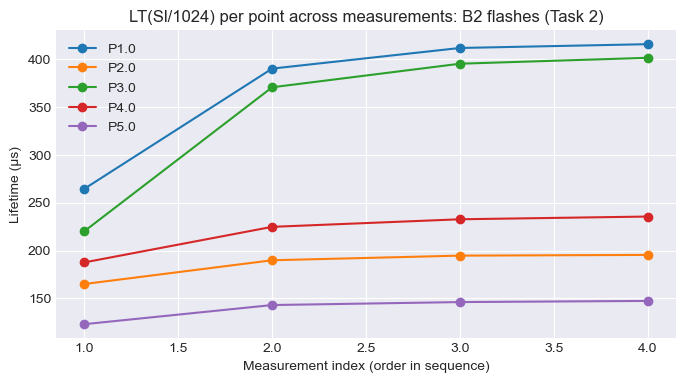
\includegraphics[width=0.6\linewidth]{plots/t2_saturate.png}
    \caption{Lifetime saturation after repeated flashes (Task 2).}
    \label{fig:t2_saturate}
\end{figure}

\begin{table}[H]
\centering
\caption{Iron constant $C_{\mu\mathrm{PCD}}$ statistics on B2 (cm$^{3}\,\mu$s).}
\begin{tabular}{lrrrr}
\toprule
Method & Value & Count & SE & boot\_hw \\
\midrule
raw\_mean      & $2.840602\times10^{13}$ & 4328 & $4.162530\times10^{13}$ & $6.762436\times10^{13}$ \\
raw\_median    & $7.025753\times10^{13}$ & 4328 & $3.631816\times10^{11}$ & $9.724196\times10^{11}$ \\
filt\_mean     & $7.649321\times10^{13}$ & 4165 & $4.064835\times10^{12}$ & $7.534944\times10^{12}$ \\
filt\_median   & $7.145814\times10^{13}$ & 4165 & $3.451062\times10^{11}$ & $9.414412\times10^{11}$ \\
trimmed\_mean  & $6.833728\times10^{13}$ & 4081 & $4.901219\times10^{11}$ & $9.575934\times10^{11}$ \\
trimmed\_median& $7.145814\times10^{13}$ & 4081 & $3.378766\times10^{11}$ & $9.544343\times10^{11}$ \\
\bottomrule
\end{tabular}
\label{tab:Cstats}
\end{table}

\begin{table}[H]
\centering
\caption{Iron concentration $N_{\mathrm{Fe}}$ statistics on B2 (cm$^{-3}$).}
\begin{tabular}{lrrrr}
\toprule
Method & Value & Count & SE & boot\_hw \\
\midrule
raw\_mean      & $6.051527\times10^{10}$ & 4294 & $3.828387\times10^{09}$ & $7.492122\times10^{09}$ \\
raw\_median    & $1.780841\times10^{10}$ & 4294 & $3.799657\times10^{08}$ & $1.202276\times10^{09}$ \\
filt\_mean     & $8.212931\times10^{10}$ & 2906 & $3.783353\times10^{09}$ & $7.452658\times10^{09}$ \\
filt\_median   & $2.812276\times10^{10}$ & 2906 & $2.752516\times10^{08}$ & $6.696133\times10^{08}$ \\
trimmed\_mean  & $6.840484\times10^{10}$ & 2846 & $2.723208\times10^{09}$ & $5.323969\times10^{09}$ \\
trimmed\_median& $2.812276\times10^{10}$ & 2846 & $2.701389\times10^{08}$ & $6.668192\times10^{08}$ \\
\bottomrule
\end{tabular}
\label{tab:NFestats}
\end{table}

\subsection{Fe--B re-association kinetics (Task 5)}
Five-point SLX series (paired state plus 0--40\,min re-association) were evaluated per point using the trimmed-median $C_{\mu\mathrm{PCD}}$. The Fe$_i$(t) decay yielded $R=3.047\times10^{-3}\,\mathrm{min^{-1}}$ ($5.078\times10^{-5}\,\mathrm{s^{-1}}$) with $R^2=0.9822$ (log-fit), Fig.~\ref{fig:task5}. Without $N_B$ we report $D_0$ for plausible boron levels:

\begin{table}[H]
\centering
\caption{Computed $D_0$ for assumed $N_B$.}
\begin{tabular}{lr}
\toprule
$N_B$ (cm$^{-3}$) & $D_0$ (cm$^{2}$/s) \\
\midrule
$1.0\times10^{15}$ & $4.79\times10^{-4}$ \\
$3.0\times10^{15}$ & $1.60\times10^{-4}$ \\
$1.0\times10^{16}$ & $4.80\times10^{-5}$ \\
$3.0\times10^{16}$ & $1.60\times10^{-5}$ \\
$1.0\times10^{17}$ & $4.97\times10^{-6}$ \\
\bottomrule
\end{tabular}
\label{tab:D0}
\end{table}

\begin{figure}[H]
    \centering
    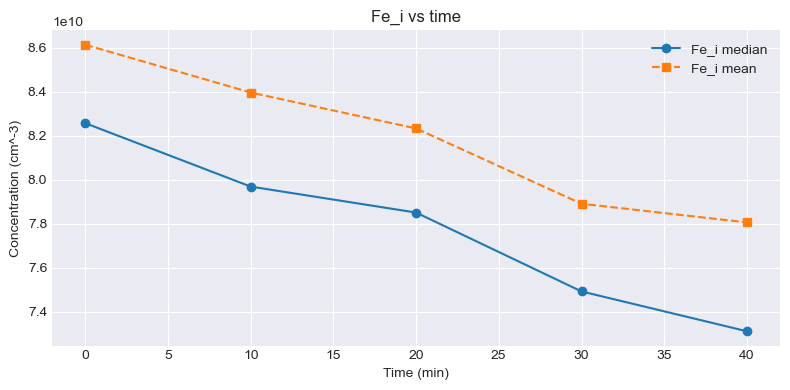
\includegraphics[width=0.6\linewidth]{plots/task5.png}
    \caption{Fe$_i$ / FeB time series and exponential fit for re-association (Task 5).}
    \label{fig:task5}
\end{figure}

\subsection{Eddy-current and laser calibration (Tasks 6--8)}
Calibration wafers produced $V_{\text{offset}}=1.2123\,\mathrm{V}$, slope $0.8375\,\mathrm{S/V}$, intercept $-1.0153\,\mathrm{S}$ with $R^2=0.9985$ (Fig.~\ref{fig:task6}). Slug calibration (2\% voltage uncertainty) after excluding the first two points gave slope $-0.69947$, intercept $1.39666$, $R^2=0.99862$ (Fig.~\ref{fig:task7}). Task 8 (laser power) was not executed during the session.

\begin{figure}[H]
    \centering
    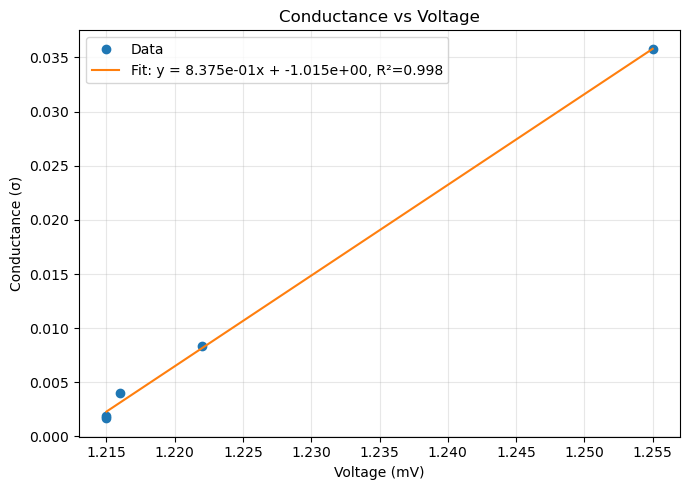
\includegraphics[width=0.6\linewidth]{plots/task6.png}
    \caption{Eddy-current calibration on wafers (Task 6).}
    \label{fig:task6}
\end{figure}

\begin{figure}[H]
    \centering
    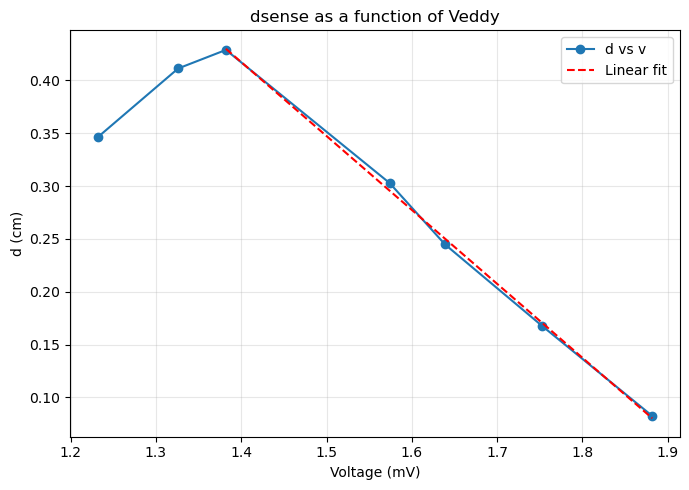
\includegraphics[width=0.6\linewidth]{plots/task7_fit.png}
    \caption{Slug calibration fit with outlier exclusion (Task 7).}
    \label{fig:task7}
\end{figure}

\subsection{Passivated wafers: $\tau(\Delta n)$ from ePCD vs SS (Tasks 9--10)}
Two passivated n-type wafers were analyzed: kx64-b1-\#449 (151\,\textmu m, $N_{\mathrm{dop}}=2.78\times10^{15}\,\mathrm{cm^{-3}}$) and kx64-b1-615 (153\,\textmu m, $1.70\times10^{15}\,\mathrm{cm^{-3}}$). Averaging ($\text{avg\_num}=512$) and Savitzky--Golay smoothing reduced noise before differentiation. The iterative mobility model provided self-consistent $\Delta n$ for each transient. Figure~\ref{fig:tau_t_passivated} compares lifetime transients at multiple pulse energies; Fig.~\ref{fig:tau_dn_passivated} shows the resulting $\tau(\Delta n)$.

\begin{figure}[H]
    \centering
    \begin{subfigure}[b]{0.48\linewidth}
        \centering
        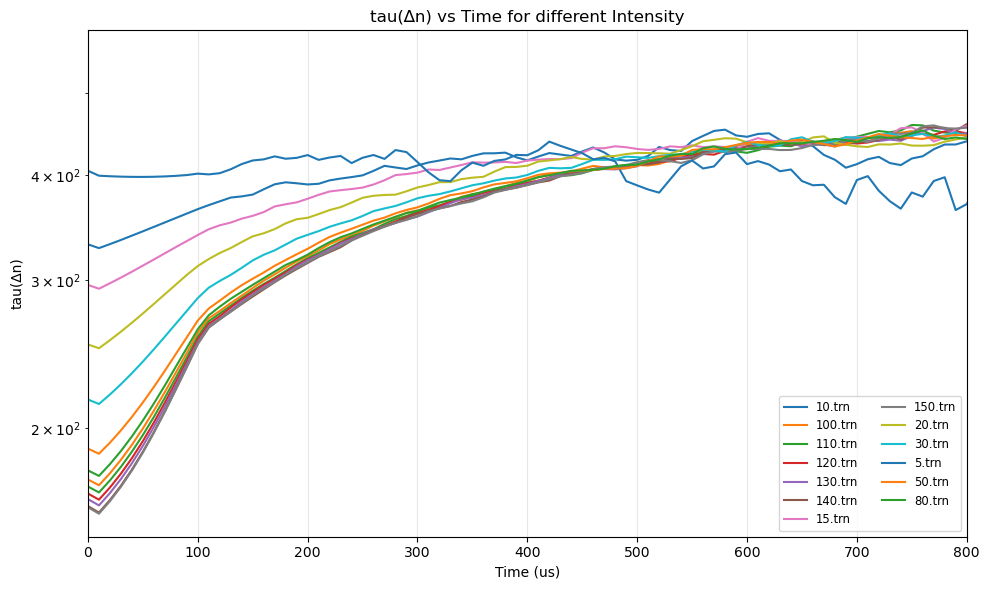
\includegraphics[width=\linewidth]{plots/tau_t_second_different_intensity.png}
        \caption{Wafer kx64-b1-\#449}
    \end{subfigure}\hfill
    \begin{subfigure}[b]{0.48\linewidth}
        \centering
        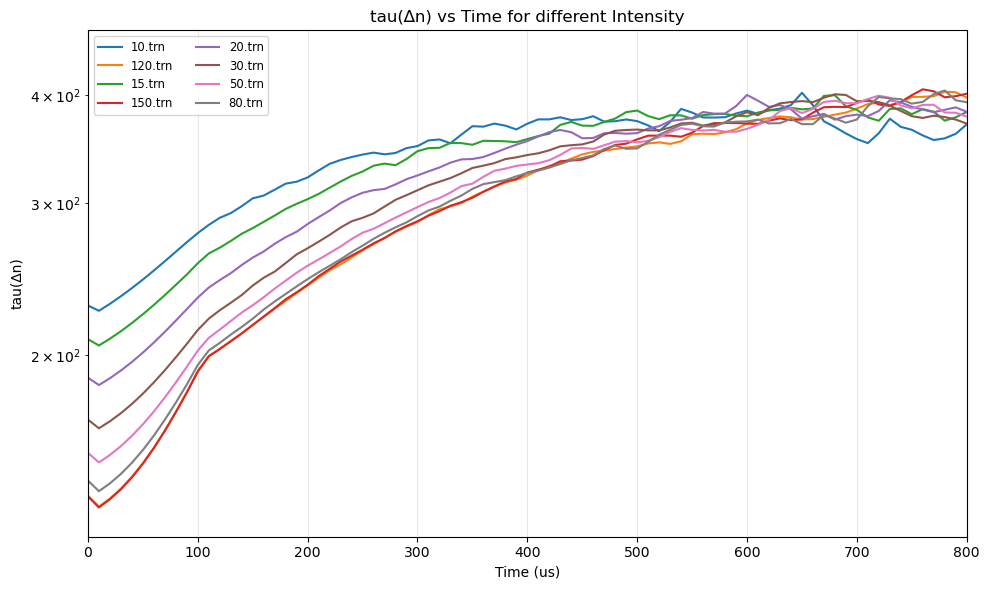
\includegraphics[width=\linewidth]{plots/tau_t_third_different_intensity.png}
        \caption{Wafer kx64-b1-615}
    \end{subfigure}

    \caption{Lifetime transients for different pulse energies (Tasks 9--10).}
    \label{fig:tau_t_passivated}
\end{figure}

\begin{figure}[H]
    \centering
    \begin{subfigure}[b]{0.48\linewidth}
        \centering
        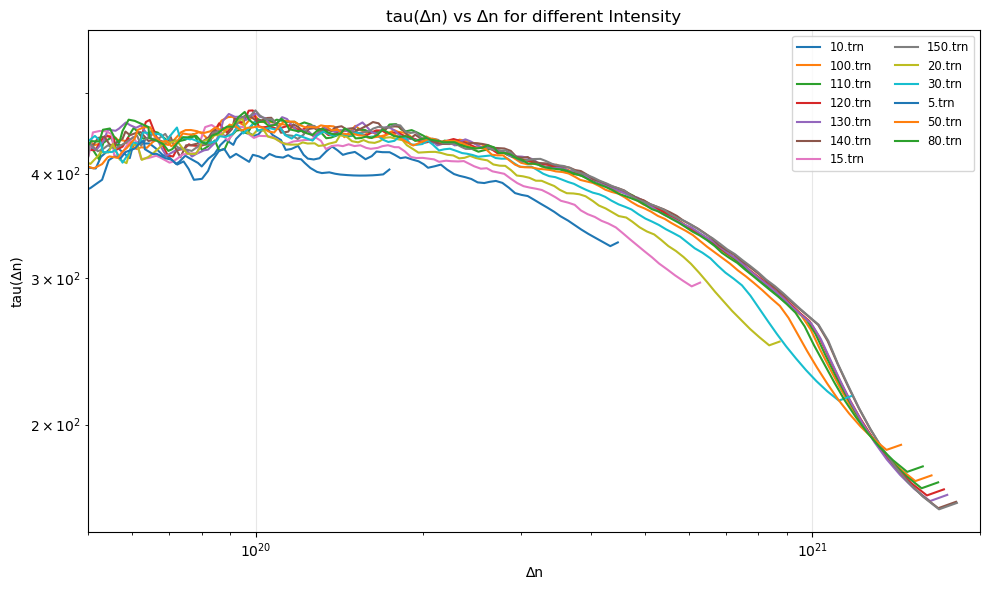
\includegraphics[width=\linewidth]{plots/tau_dn_second_different_intensity.png}
        \caption{Wafer kx64-b1-\#449}
    \end{subfigure}\hfill
    \begin{subfigure}[b]{0.48\linewidth}
        \centering
        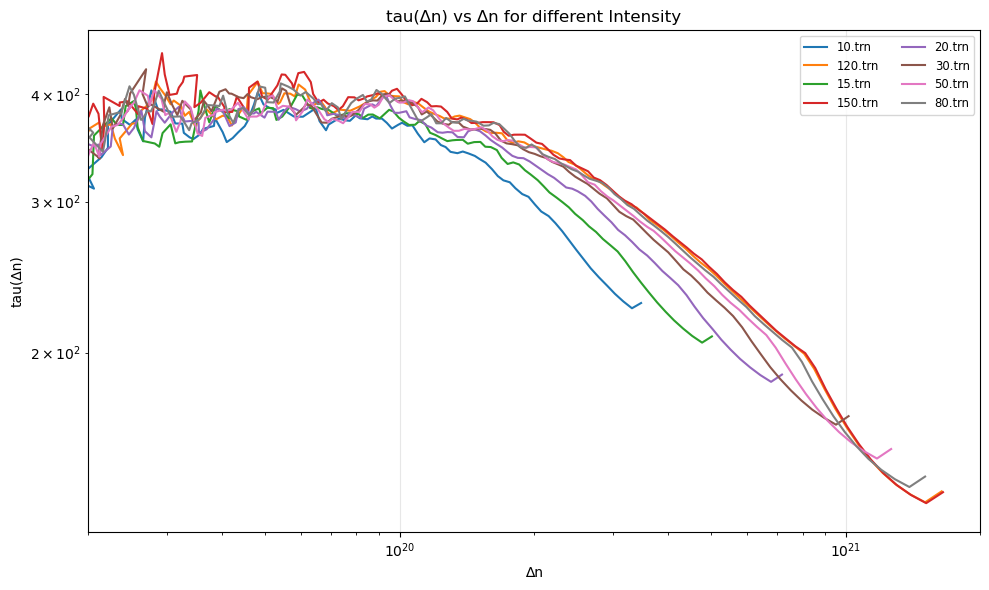
\includegraphics[width=\linewidth]{plots/tau_dn_third_different_intensity.png}
        \caption{Wafer kx64-b1-615}
    \end{subfigure}

    \caption{$\tau(\Delta n)$ derived from ePCD/SS comparison (Tasks 9--10).}
    \label{fig:tau_dn_passivated}
\end{figure}

\subsection{Ingots: thickness and surface recombination (Tasks 12--13)}
Injection-dependent decay was recorded on thick ingots (kx78: 2.40, 0.92, 0.74, 0.64\,cm; kx77: 2.52, 0.99, 0.64, 0.70\,cm). Base DC voltages were 1.696\,V (kx78) and 1.373\,V (kx77) for conductance baselines. Sensitivity depth $d_{\text{sense}}=\rho/\sigma_{\text{sh,app}}$ set the effective thickness for unpassivated pieces. Figures compile $\Delta n(t)$ and $\tau(\Delta n)$ under varying pulse intensity and width. Surface recombination dominates the thinner, unpassivated slugs, while thicker samples retain longer decay tails consistent with diffusion limitation.

\begin{figure}[H]
    \centering
    \begin{subfigure}[b]{0.48\linewidth}
        \centering
        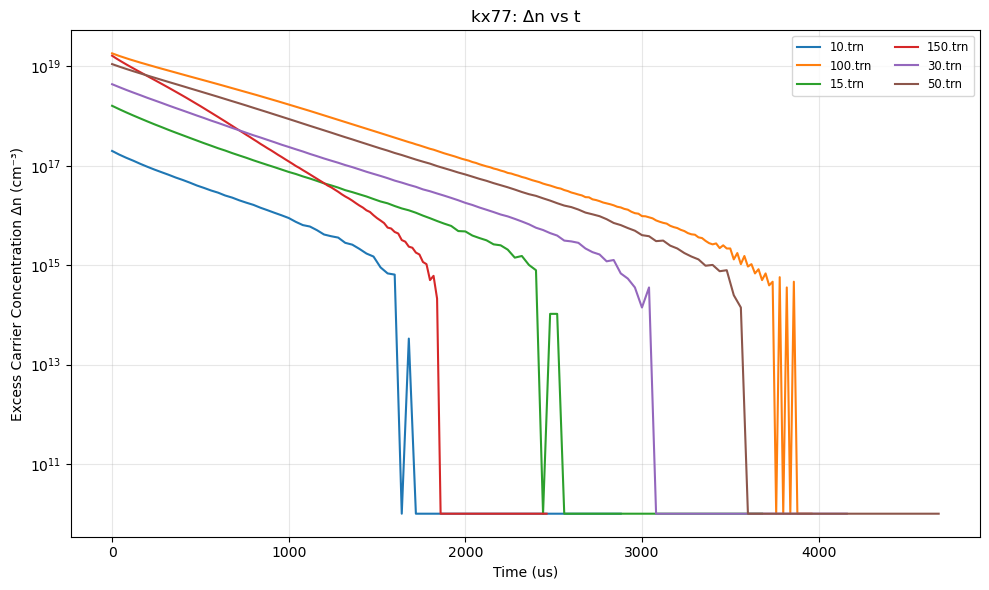
\includegraphics[width=\linewidth]{plots/dn_t_kx77_first_different_intensity.png}
        \caption{kx77, varying intensity}
    \end{subfigure}\hfill
    \begin{subfigure}[b]{0.48\linewidth}
        \centering
        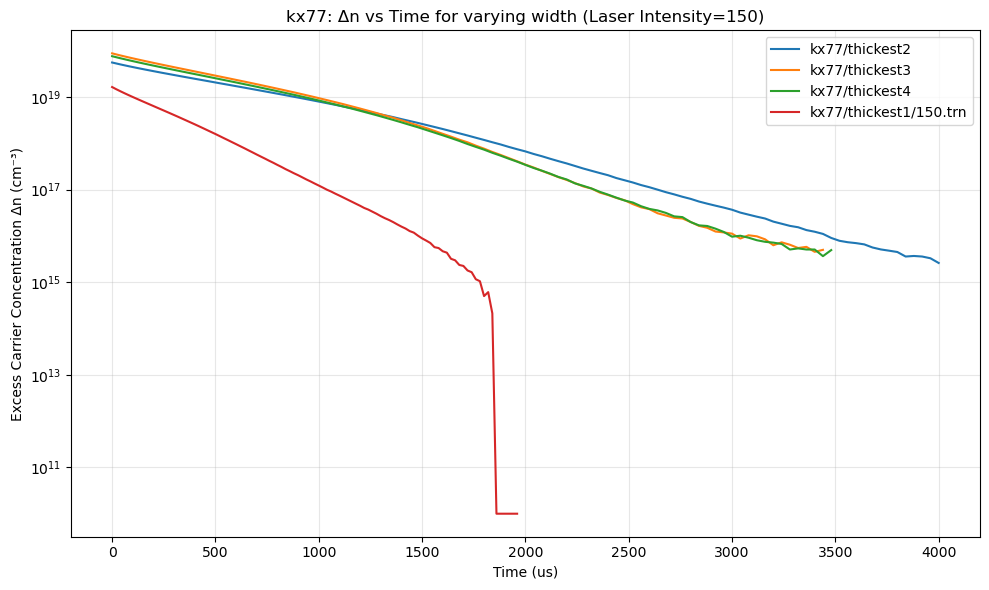
\includegraphics[width=\linewidth]{plots/dn_t_kx77_first_different_width.png}
        \caption{kx77, varying width}
    \end{subfigure}

    \caption{$\Delta n(t)$ for kx77 ingots (Task 12).}
    \label{fig:dn_t_kx77}
\end{figure}

\begin{figure}[H]
    \centering
    \begin{subfigure}[b]{0.48\linewidth}
        \centering
        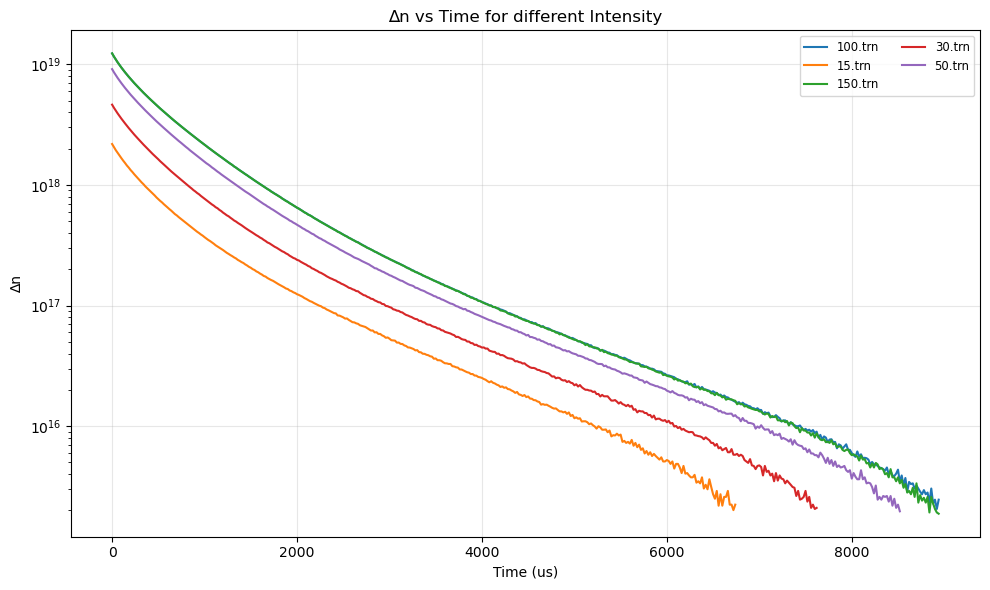
\includegraphics[width=\linewidth]{plots/dn_t_kx78_first_different_intensity.png}
        \caption{kx78, varying intensity}
    \end{subfigure}\hfill
    \begin{subfigure}[b]{0.48\linewidth}
        \centering
        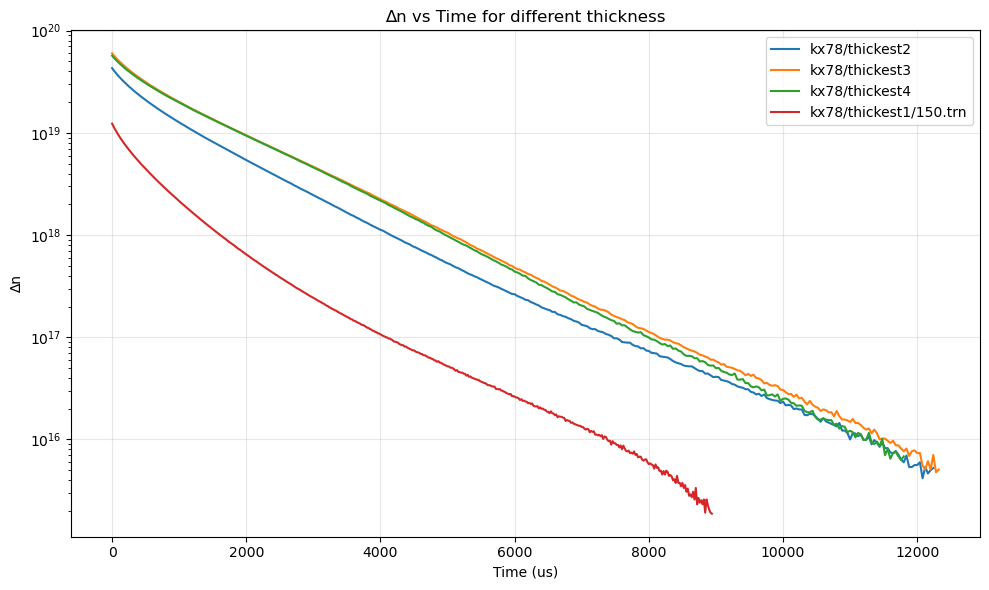
\includegraphics[width=\linewidth]{plots/dn_t_kx78_first_different_width.png}
        \caption{kx78, varying width}
    \end{subfigure}

    \caption{$\Delta n(t)$ for kx78 ingots (Task 12).}
    \label{fig:dn_t_kx78}
\end{figure}

\begin{figure}[H]
    \centering
    \begin{subfigure}[b]{0.48\linewidth}
        \centering
        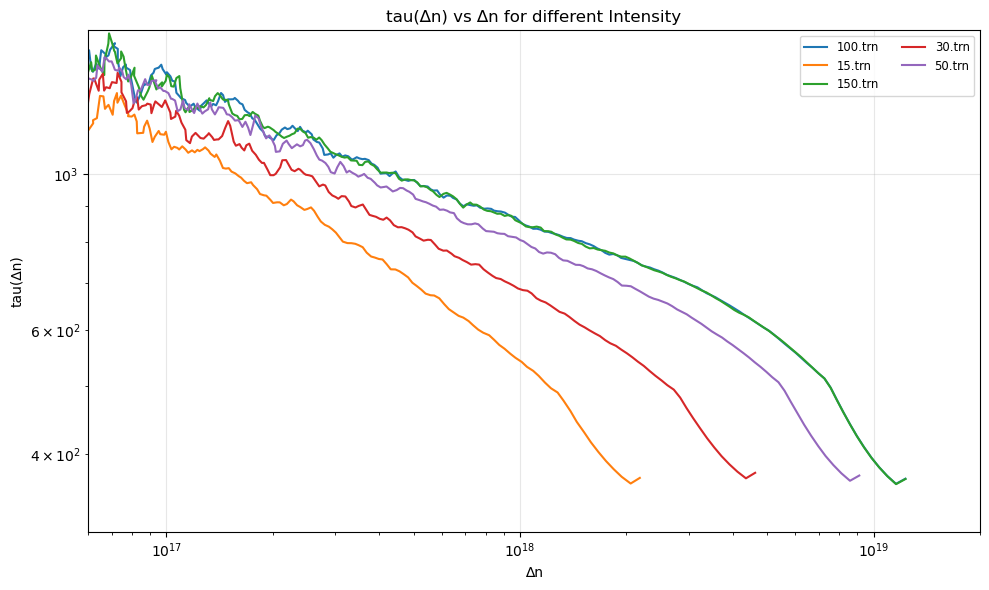
\includegraphics[width=\linewidth]{plots/tau_dn_k78_different_intensity.png}
        \caption{kx78, varying intensity}
    \end{subfigure}\hfill
    \begin{subfigure}[b]{0.48\linewidth}
        \centering
        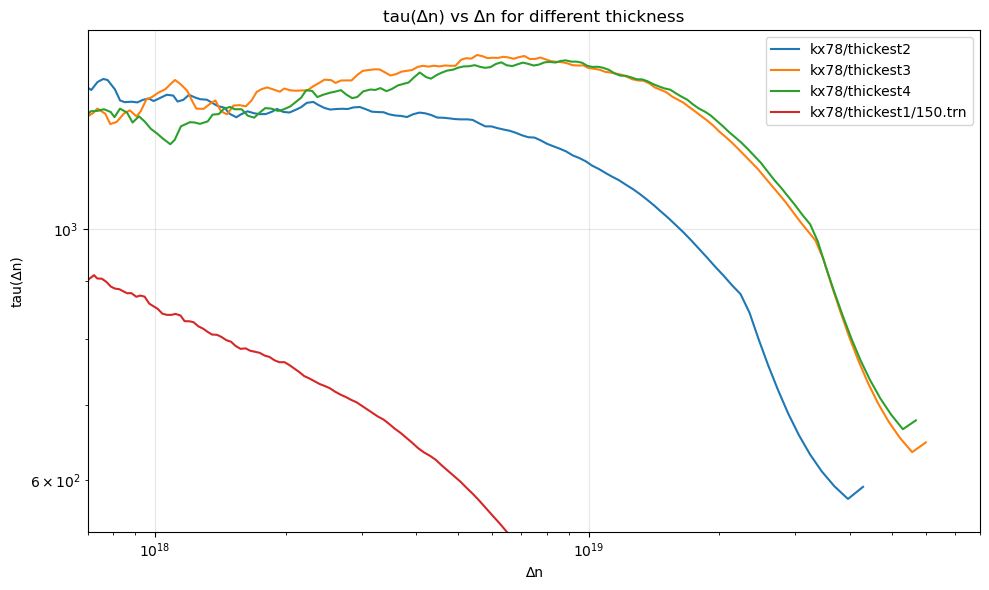
\includegraphics[width=\linewidth]{plots/tau_dn_k78_different_width.png}
        \caption{kx78, varying width}
    \end{subfigure}

    \caption{$\tau(\Delta n)$ for kx78 ingots (Task 12).}
    \label{fig:tau_dn_kx78}
\end{figure}

\begin{figure}[H]
    \centering
    \begin{subfigure}[b]{0.48\linewidth}
        \centering
        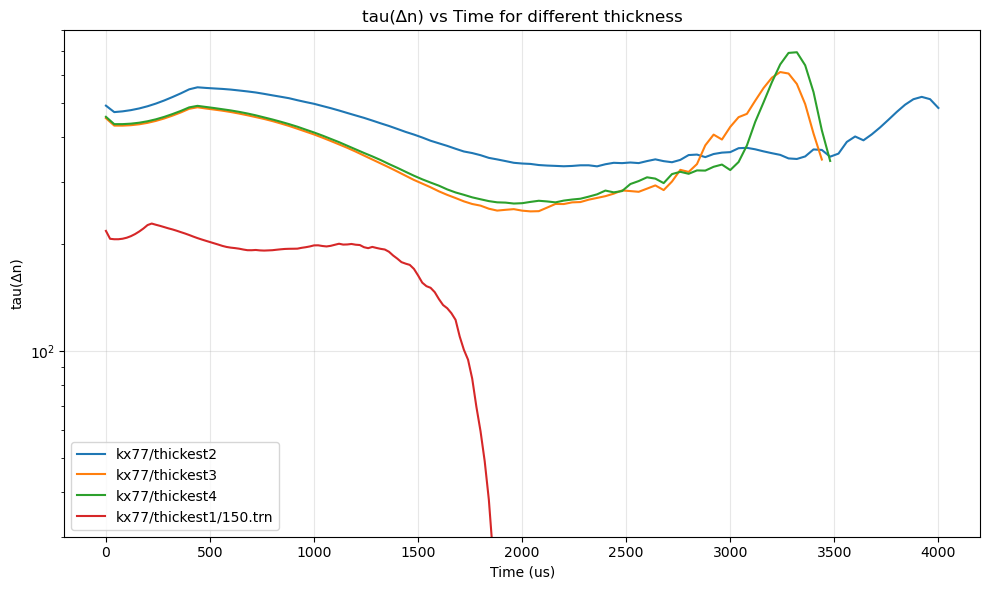
\includegraphics[width=\linewidth]{plots/tau_t_kx77_different_width.png}
        \caption{kx77, varying width}
    \end{subfigure}\hfill
    \begin{subfigure}[b]{0.48\linewidth}
        \centering
        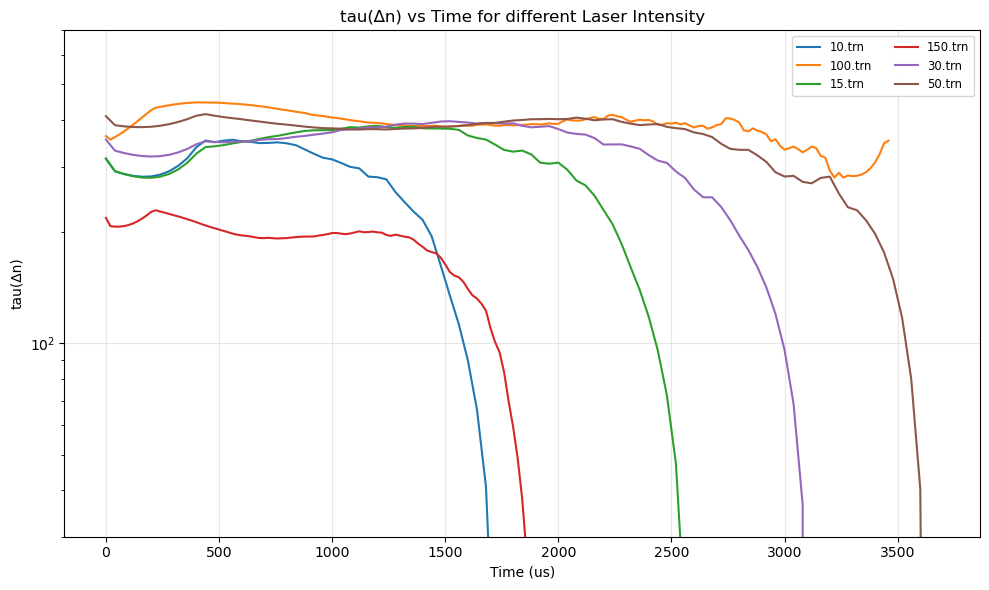
\includegraphics[width=\linewidth]{plots/tau_t_kx77_first_different_intensity.png}
        \caption{kx77, varying intensity}
    \end{subfigure}

    \caption{Lifetime transients $\tau(t)$ for kx77 ingots (Task 13).}
    \label{fig:tau_t_kx77}
\end{figure}

\begin{figure}[H]
    \centering
    \begin{subfigure}[b]{0.48\linewidth}
        \centering
        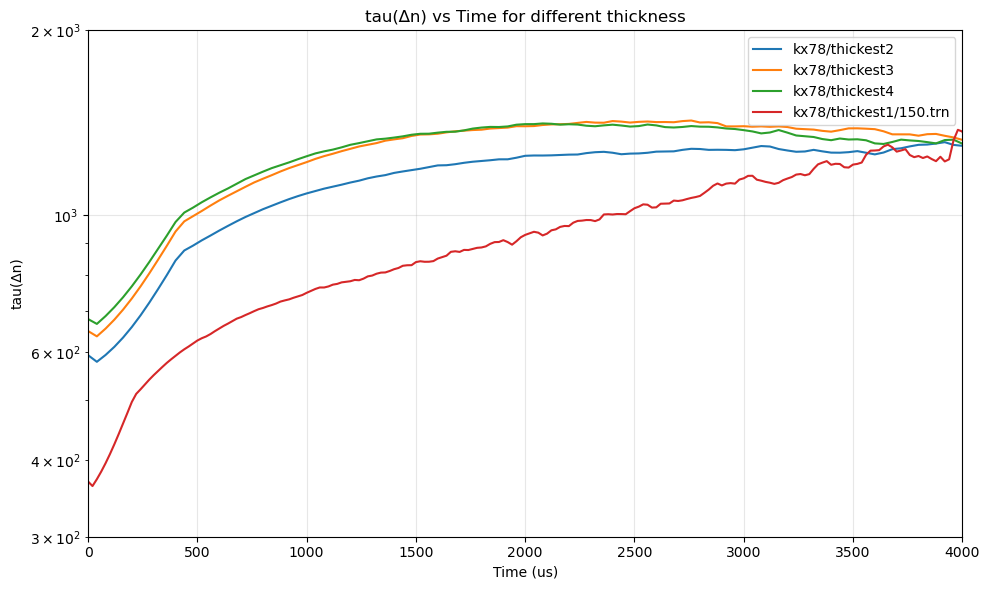
\includegraphics[width=\linewidth]{plots/tau_t_kx78_different_width.png}
        \caption{kx78, varying width}
    \end{subfigure}\hfill
    \begin{subfigure}[b]{0.48\linewidth}
        \centering
        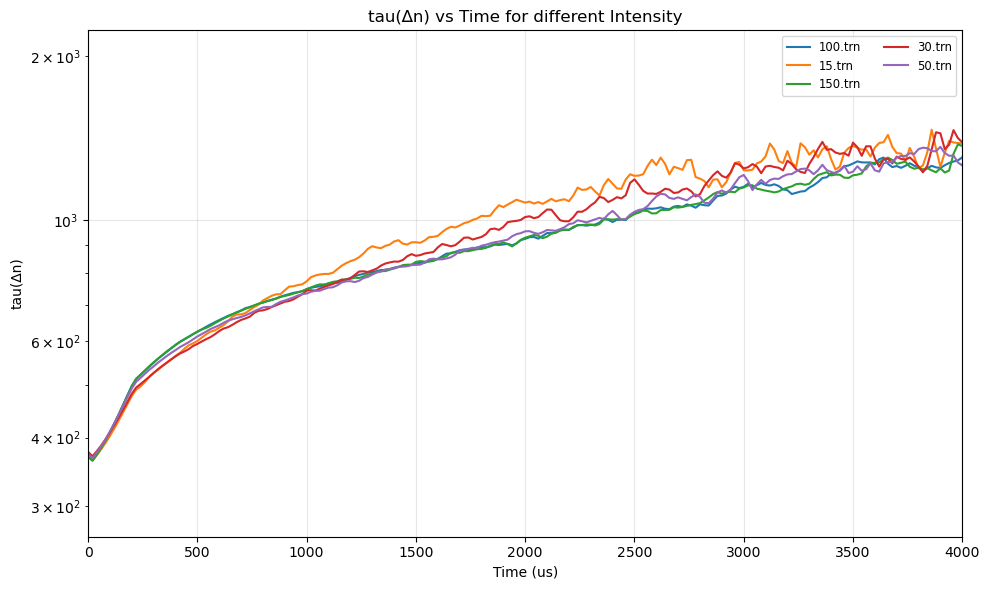
\includegraphics[width=\linewidth]{plots/tau_t_kx78_first_different_intensity.png}
        \caption{kx78, varying intensity}
    \end{subfigure}

    \caption{Lifetime transients $\tau(t)$ for kx78 ingots (Task 13).}
    \label{fig:tau_t_kx78}
\end{figure}

% Conclusion
\section{Conclusion}
Robust per-pixel processing of μPCD maps delivered an iron constant of $7.15\times10^{13}\,\mathrm{cm^{3}\,\mu s}$ and Fe concentration of $2.81\times10^{10}\,\mathrm{cm^{-3}}$ on the reference wafer, with flash saturation verified experimentally. Fe--B re-association followed a single-exponential kinetics with $R=5.08\times10^{-5}\,\mathrm{s^{-1}}$; candidate $D_0$ values are reported pending boron concentration. Eddy-current calibration achieved sub-percent linearity and provided the baseline for injection-level reconstructions. Passivated wafers showed stable $\tau(\Delta n)$ after smoothing and iterative mobility corrections, while thick ingots exhibited thickness- and surface-driven lifetime reductions at low injection, consistent with surface recombination limits. Future refinement requires the boron concentration (or resistivity) for $D_0$ closure and laser power calibration (Task 8).

\end{document}

